% Options for packages loaded elsewhere
\PassOptionsToPackage{unicode}{hyperref}
\PassOptionsToPackage{hyphens}{url}
%
\documentclass[
]{book}
\usepackage{amsmath,amssymb}
\usepackage{iftex}
\ifPDFTeX
  \usepackage[T1]{fontenc}
  \usepackage[utf8]{inputenc}
  \usepackage{textcomp} % provide euro and other symbols
\else % if luatex or xetex
  \usepackage{unicode-math} % this also loads fontspec
  \defaultfontfeatures{Scale=MatchLowercase}
  \defaultfontfeatures[\rmfamily]{Ligatures=TeX,Scale=1}
\fi
\usepackage{lmodern}
\ifPDFTeX\else
  % xetex/luatex font selection
\fi
% Use upquote if available, for straight quotes in verbatim environments
\IfFileExists{upquote.sty}{\usepackage{upquote}}{}
\IfFileExists{microtype.sty}{% use microtype if available
  \usepackage[]{microtype}
  \UseMicrotypeSet[protrusion]{basicmath} % disable protrusion for tt fonts
}{}
\makeatletter
\@ifundefined{KOMAClassName}{% if non-KOMA class
  \IfFileExists{parskip.sty}{%
    \usepackage{parskip}
  }{% else
    \setlength{\parindent}{0pt}
    \setlength{\parskip}{6pt plus 2pt minus 1pt}}
}{% if KOMA class
  \KOMAoptions{parskip=half}}
\makeatother
\usepackage{xcolor}
\usepackage{color}
\usepackage{fancyvrb}
\newcommand{\VerbBar}{|}
\newcommand{\VERB}{\Verb[commandchars=\\\{\}]}
\DefineVerbatimEnvironment{Highlighting}{Verbatim}{commandchars=\\\{\}}
% Add ',fontsize=\small' for more characters per line
\usepackage{framed}
\definecolor{shadecolor}{RGB}{248,248,248}
\newenvironment{Shaded}{\begin{snugshade}}{\end{snugshade}}
\newcommand{\AlertTok}[1]{\textcolor[rgb]{0.94,0.16,0.16}{#1}}
\newcommand{\AnnotationTok}[1]{\textcolor[rgb]{0.56,0.35,0.01}{\textbf{\textit{#1}}}}
\newcommand{\AttributeTok}[1]{\textcolor[rgb]{0.13,0.29,0.53}{#1}}
\newcommand{\BaseNTok}[1]{\textcolor[rgb]{0.00,0.00,0.81}{#1}}
\newcommand{\BuiltInTok}[1]{#1}
\newcommand{\CharTok}[1]{\textcolor[rgb]{0.31,0.60,0.02}{#1}}
\newcommand{\CommentTok}[1]{\textcolor[rgb]{0.56,0.35,0.01}{\textit{#1}}}
\newcommand{\CommentVarTok}[1]{\textcolor[rgb]{0.56,0.35,0.01}{\textbf{\textit{#1}}}}
\newcommand{\ConstantTok}[1]{\textcolor[rgb]{0.56,0.35,0.01}{#1}}
\newcommand{\ControlFlowTok}[1]{\textcolor[rgb]{0.13,0.29,0.53}{\textbf{#1}}}
\newcommand{\DataTypeTok}[1]{\textcolor[rgb]{0.13,0.29,0.53}{#1}}
\newcommand{\DecValTok}[1]{\textcolor[rgb]{0.00,0.00,0.81}{#1}}
\newcommand{\DocumentationTok}[1]{\textcolor[rgb]{0.56,0.35,0.01}{\textbf{\textit{#1}}}}
\newcommand{\ErrorTok}[1]{\textcolor[rgb]{0.64,0.00,0.00}{\textbf{#1}}}
\newcommand{\ExtensionTok}[1]{#1}
\newcommand{\FloatTok}[1]{\textcolor[rgb]{0.00,0.00,0.81}{#1}}
\newcommand{\FunctionTok}[1]{\textcolor[rgb]{0.13,0.29,0.53}{\textbf{#1}}}
\newcommand{\ImportTok}[1]{#1}
\newcommand{\InformationTok}[1]{\textcolor[rgb]{0.56,0.35,0.01}{\textbf{\textit{#1}}}}
\newcommand{\KeywordTok}[1]{\textcolor[rgb]{0.13,0.29,0.53}{\textbf{#1}}}
\newcommand{\NormalTok}[1]{#1}
\newcommand{\OperatorTok}[1]{\textcolor[rgb]{0.81,0.36,0.00}{\textbf{#1}}}
\newcommand{\OtherTok}[1]{\textcolor[rgb]{0.56,0.35,0.01}{#1}}
\newcommand{\PreprocessorTok}[1]{\textcolor[rgb]{0.56,0.35,0.01}{\textit{#1}}}
\newcommand{\RegionMarkerTok}[1]{#1}
\newcommand{\SpecialCharTok}[1]{\textcolor[rgb]{0.81,0.36,0.00}{\textbf{#1}}}
\newcommand{\SpecialStringTok}[1]{\textcolor[rgb]{0.31,0.60,0.02}{#1}}
\newcommand{\StringTok}[1]{\textcolor[rgb]{0.31,0.60,0.02}{#1}}
\newcommand{\VariableTok}[1]{\textcolor[rgb]{0.00,0.00,0.00}{#1}}
\newcommand{\VerbatimStringTok}[1]{\textcolor[rgb]{0.31,0.60,0.02}{#1}}
\newcommand{\WarningTok}[1]{\textcolor[rgb]{0.56,0.35,0.01}{\textbf{\textit{#1}}}}
\usepackage{longtable,booktabs,array}
\usepackage{calc} % for calculating minipage widths
% Correct order of tables after \paragraph or \subparagraph
\usepackage{etoolbox}
\makeatletter
\patchcmd\longtable{\par}{\if@noskipsec\mbox{}\fi\par}{}{}
\makeatother
% Allow footnotes in longtable head/foot
\IfFileExists{footnotehyper.sty}{\usepackage{footnotehyper}}{\usepackage{footnote}}
\makesavenoteenv{longtable}
\usepackage{graphicx}
\makeatletter
\def\maxwidth{\ifdim\Gin@nat@width>\linewidth\linewidth\else\Gin@nat@width\fi}
\def\maxheight{\ifdim\Gin@nat@height>\textheight\textheight\else\Gin@nat@height\fi}
\makeatother
% Scale images if necessary, so that they will not overflow the page
% margins by default, and it is still possible to overwrite the defaults
% using explicit options in \includegraphics[width, height, ...]{}
\setkeys{Gin}{width=\maxwidth,height=\maxheight,keepaspectratio}
% Set default figure placement to htbp
\makeatletter
\def\fps@figure{htbp}
\makeatother
\setlength{\emergencystretch}{3em} % prevent overfull lines
\providecommand{\tightlist}{%
  \setlength{\itemsep}{0pt}\setlength{\parskip}{0pt}}
\setcounter{secnumdepth}{5}
\usepackage{booktabs}
\usepackage{amsthm}
\makeatletter
\def\thm@space@setup{%
  \thm@preskip=8pt plus 2pt minus 4pt
  \thm@postskip=\thm@preskip
}
\makeatother
\ifLuaTeX
  \usepackage{selnolig}  % disable illegal ligatures
\fi
\usepackage[]{natbib}
\bibliographystyle{apalike}
\IfFileExists{bookmark.sty}{\usepackage{bookmark}}{\usepackage{hyperref}}
\IfFileExists{xurl.sty}{\usepackage{xurl}}{} % add URL line breaks if available
\urlstyle{same}
\hypersetup{
  pdftitle={A Minimal Book Example},
  pdfauthor={Yihui Xie},
  hidelinks,
  pdfcreator={LaTeX via pandoc}}

\title{A Minimal Book Example}
\author{Yihui Xie}
\date{2024-04-25}

\begin{document}
\maketitle

{
\setcounter{tocdepth}{1}
\tableofcontents
}
\hypertarget{prerequisites}{%
\chapter{Prerequisites}\label{prerequisites}}

This is a \emph{sample} book written in \textbf{Markdown}. You can use anything that Pandoc's Markdown supports, e.g., a math equation \(a^2 + b^2 = c^2\).

The \textbf{bookdown} package can be installed from CRAN or Github:

\begin{Shaded}
\begin{Highlighting}[]
\FunctionTok{install.packages}\NormalTok{(}\StringTok{"bookdown"}\NormalTok{)}
\CommentTok{\# or the development version}
\CommentTok{\# devtools::install\_github("rstudio/bookdown")}
\end{Highlighting}
\end{Shaded}

Remember each Rmd file contains one and only one chapter, and a chapter is defined by the first-level heading \texttt{\#}.

To compile this example to PDF, you need XeLaTeX. You are recommended to install TinyTeX (which includes XeLaTeX): \url{https://yihui.name/tinytex/}.

\hypertarget{introductie}{%
\chapter{Introductie}\label{introductie}}

\hypertarget{cv}{%
\chapter{CV}\label{cv}}

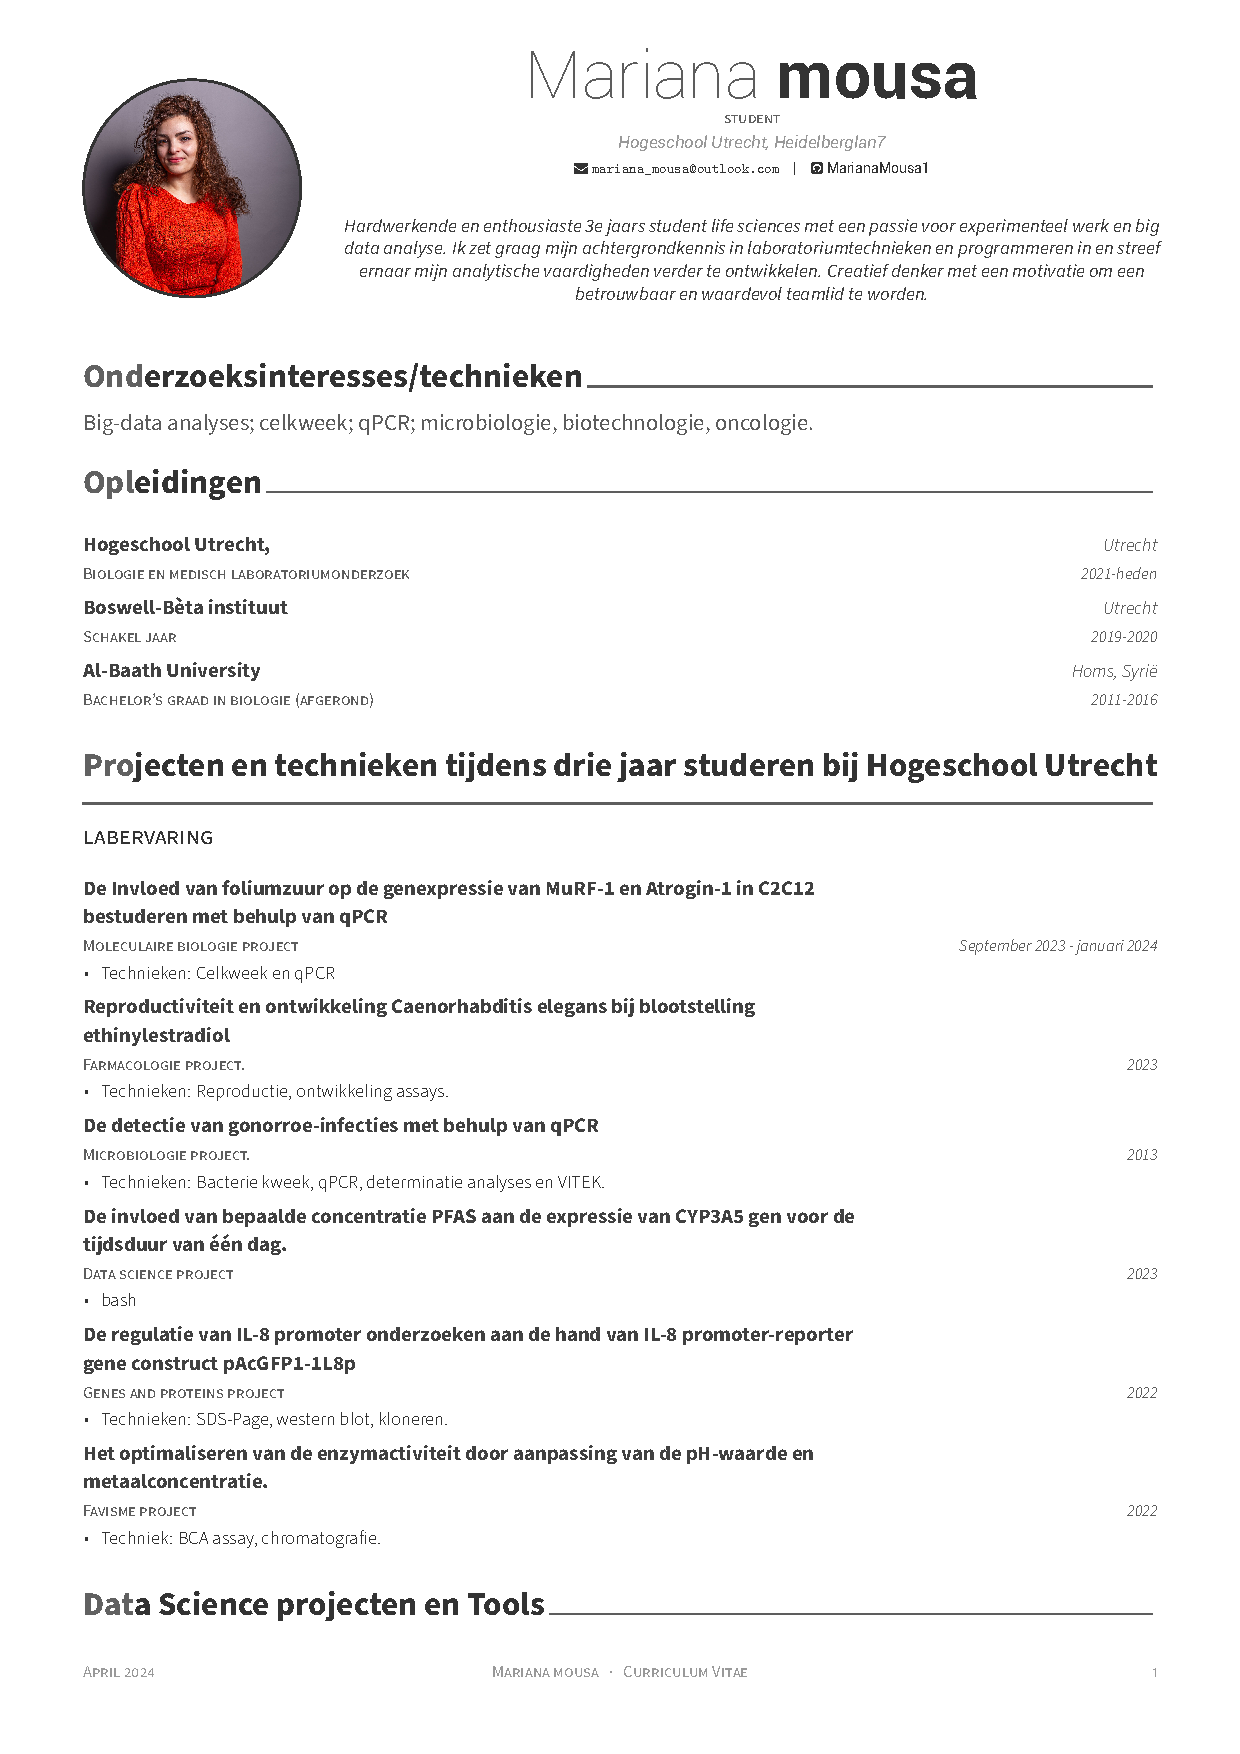
\includegraphics[width=1\linewidth,height=1000]{MarianaCV}

\hypertarget{vooruit-kijken}{%
\chapter{vooruit kijken}\label{vooruit-kijken}}

\begin{itemize}
\item
  Over twee jaar zie ik mezelf graag mijn vaardigheden en kennis op het gebied van de data science en life science verder ontwikkelen. Daarom overweeg ik om een Master Projectmanagement te volgen om mijn expertise te vergroten en mijn carrière vooruit te helpen.
\item
  In de toekomst wil ik graag mijn kennis in de wetenschap gebruiken om de kwaliteit van het leven van de mensen in het algemeen en specifiek van de patienten verbeteren door het begeleiden van onderzoeks projecten.
\item
  Op dit moment ben ik actief bezig met het vergroten van mijn kennis en vaardigheden om de projecten goed te kunnen regelen en duidelijke plannen maken.
\item
  De volgende vaardigheid die ik graag zou willen leren naast leiderschapsvaardigheid, is het uitvoeren van NGS-analyses en het beheersen van HLA-typing R-tools om de genetische variaties te bestuderen die verband houden met ziekten, zoals kanker, auto-immuunziekten en genetische aandoeningen. Dit kan leiden tot een dieper inzicht in de oorzaken van ziekten en nieuwe behandelingsmogelijkheden.
\end{itemize}

\hypertarget{vrijruimte-opdracht}{%
\chapter{vrijruimte opdracht}\label{vrijruimte-opdracht}}

paper
hlaR: A rapid and reproducible tool to identify eplet mismatches between transplant donors and recipients

Introduction

HLA-typering, ook bekend als HLA-genotypering of HLA-typing, is een laboratoriumtechniek die wordt gebruikt om de genetische varianten van de menselijke leukocytenantigeen (HLA)-genen in een individu te identificeren. HLA-genen coderen voor eiwitten die zich op het celoppervlak bevinden en een cruciale rol spelen bij het immuunsysteem door het lichaam te helpen onderscheid te maken tussen eigen cellen en indringers zoals bacteriën en virussen.

Het menselijke HLA-systeem is zeer polymorf, wat betekent dat er veel verschillende varianten (allelen) van HLA-genen zijn die tussen individuen kunnen verschillen. Deze genetische variabiliteit speelt een belangrijke rol bij het bepalen van de compatibiliteit van weefsels en organen voor transplantatie, evenals bij het risico op auto-immuunziekten, allergieën en andere immuungerelateerde aandoeningen.

HLA-typering omvat het identificeren van de specifieke allelen van HLA-klasse I-genen (HLA-A, HLA-B en HLA-C) en HLA-klasse II-genen (HLA-DR, HLA-DQ en HLA-DP) in een individu. Dit kan worden gedaan met behulp van verschillende laboratoriumtechnieken, waaronder moleculaire methoden zoals polymerasekettingreactie (PCR) gevolgd door sequentieanalyse, next-generation sequencing (NGS), en andere gespecialiseerde technieken.

HLA-typering is essentieel bij transplantatiegeneeskunde omdat een goede match tussen donor en ontvanger op HLA-allelen het risico op afstoting van getransplanteerde weefsels en organen vermindert. Het wordt ook gebruikt bij het onderzoek naar immuungerelateerde aandoeningen om te begrijpen hoe genetische variaties in het HLA-systeem het risico op ziekte beïnvloeden.

  \bibliography{book.bib,packages.bib}

\end{document}
